% Provenance (never printed): see sources/outline_sources.md (Year 1: gravity and its
% measurement, normal gravity; isostasy, Airy and Pratt; free-air and Bouguer anomalies;
% the geoid). Curves from figdata/bachelor-1/hypsometry.py and gravity_profiles.py;
% exercise and problem values in the Book 3 scratch calculator calc/ch11.py.
\chapter{Isostasy and Gravity Anomalies}\label{ch:b1:isostasy-gravity}

In the 1840s the surveyors measuring a meridian arc across northern India met a
discrepancy they could not blame on their instruments. Between two stations
about 370 miles apart, Kaliana near the foot of the Himalaya and Kalianpur far
to the south, the difference of \omterm{def:b1:spherical-astronomy:geographic}{latitude} found by triangulation exceeded the
difference found from the stars by 5.236 seconds of arc. The obvious culprit
was the mountains: their attraction pulls a plumb line northwards, and the
astronomers set their instruments by the plumb line. In 1855 John Henry Pratt
computed the attraction of the Himalaya and of the plateaux beyond them and
found that it should have made the discrepancy 15.885 seconds, more than three
times what was observed. The mountains pulled much less than their visible mass
required. The same year George Airy answered that the \omterm{def:b1:layered-earth:layers}{crust} floats on a denser
layer like a raft of logs on water, so that high ground has a deep root of
light rock; Pratt later proposed another answer, rock made lighter by
expansion beneath the mountains. Both are still taught: the mountains are
underlain by light rock that makes up for their mass. This chapter turns that
idea into
numbers, and shows how gravity, measured to a millionth of its value, reveals
the masses hidden below the relief.
% ledger: pratt:himalaya, airy:1855, pratt:1871

\begin{recall}
Newton's law of gravitation gives the field $g = GM/r^2$ outside a spherical
mass $M$; the field derives from a gravitational potential, and an equipotential
surface is everywhere perpendicular to the field (physics). In a fluid at rest
the pressure increases with depth as $\mathrm dp/\mathrm dz = \rho g$, and a
floating body displaces its own weight of fluid (physics, University Year 1).
Below the \omterm{def:b1:layered-earth:lithosphere}{lithosphere} the \omterm{def:b1:layered-earth:lithosphere}{asthenosphere} flows over long times; the \omterm{def:b1:layered-earth:layers}{crust} is
lighter than the \omterm{def:b1:layered-earth:layers}{mantle} below it (\cref{ch:b1:layered-earth}; Book 2, grade 11).
\end{recall}

\section{Gravity and its measurement}

The acceleration of gravity at the Earth's surface is close to
\qty{9.8}{m.s^{-2}}, and the variations that interest geologists are a
million times smaller. They are counted in a unit of the old centimetre--gram
system, the gal: $\qty{1}{Gal} = \qty{1}{cm.s^{-2}} = \qty{0.01}{m.s^{-2}}$, so
that
\[
  \qty{1}{\milli\gal} = \qty{e-5}{m.s^{-2}} \approx \num{e-6}\,g .
\]
% ledger: nist:gal
A field instrument resolves a few thousandths of a milligal; the anomalies
studied in this chapter range from a fraction of a milligal over a buried ore
body to a few hundred milligals over a mountain range.

Even on a featureless Earth, gravity would not be the same everywhere. The
Earth turns, so that what a plumb line or a gravimeter feels is the sum of the
gravitational attraction and the centrifugal effect of rotation; and the
Earth is flattened, so that the poles are nearer its centre than the equator.
Both effects make gravity weaker at the equator than at the poles. A geologist
compares every measurement with a smooth reference that contains them.

\begin{definition}[Normal gravity]\label{def:b1:isostasy-gravity:normal-gravity}
\emph{Normal gravity}\index{normal gravity} $\gamma$ is the gravity of a model
Earth: an ellipsoid of revolution with the Earth's mass and rotation, chosen so
that its surface is an equipotential of its own gravity (gravitation plus the
centrifugal effect). On that surface, normal gravity depends on \omterm{def:b1:spherical-astronomy:geographic}{latitude} alone.
\end{definition}

The ellipsoid itself, its flattening and the way its parameters are fitted to
the real Earth are studied in Book 5. Here we only need its gravity.

\begin{proposition}[The normal gravity formula]\label{prop:b1:isostasy-gravity:normal-formula}
On the reference ellipsoid adopted in 1980, \omterm{def:b1:isostasy-gravity:normal-gravity}{normal gravity} at the geographic
\omterm{def:b1:spherical-astronomy:geographic}{latitude} $\varphi$ is, in its usual series form,
\[
  \gamma(\varphi) = \qty{9.780327}{m.s^{-2}}\,\bigl(1 + 0.0053024\sin^2\varphi
  - 0.0000058\sin^2 2\varphi\bigr).
\]
\end{proposition}
\admitted
% ledger: moritz:grs80

It gives \qty{9.780327}{m.s^{-2}} at the equator, \qty{9.806200}{m.s^{-2}} at
\ang{45} and \qty{9.832186}{m.s^{-2}} at the poles: a difference of
\qty{5186}{\milli\gal} from equator to pole. The rotation alone accounts for
most of it. With the sidereal day of \qty{23.9345}{h}, the angular velocity is
$\omega = 2\pi/\qty{86164}{s} = \qty{7.292e-5}{rad.s^{-1}}$, and the centrifugal
acceleration at the equator, $\omega^2 a$ with $a = \qty{6378.137}{km}$, is
\qty{0.0339}{m.s^{-2}}, or \qty{3392}{\milli\gal}; the flattening supplies the
rest (\cref{exo:b1:isostasy-gravity:2}).
% ledger: earth:Trot, earth:Req, earth:geq, earth:gpole

Gravity is measured in two ways. An \emph{absolute} gravimeter drops a test
mass in a vacuum chamber and follows its free fall with a laser interferometer,
timed by an atomic clock: the acceleration comes out directly from distance and
time. A \emph{relative} gravimeter is a mass hung on a spring, whose stretch
changes with gravity; it is light and fast, but it only gives differences
between places, and it drifts, so a survey returns to a base station whose
gravity is known. The best absolute instruments are accurate to about a
microgal, a part in a billion of $g$.
% ledger: ngs:absolute-gravity

\begin{inthefield}[A gravity survey on land]
\begin{minipage}[t]{0.55\linewidth}\vspace{0pt}
A gravity survey is a slow walk from station to station. At each one the
geophysicist sets the relative gravimeter on its tripod, levels it, waits for
the spring to settle and takes several readings; a satellite-positioning
receiver beside it records the station's position and height. Every few hours
the team goes back to the base station, so that the drift of the spring can be
measured and removed. The height matters as much as the gravity: as the next
section shows, gravity falls by \qty{0.3086}{\milli\gal} for every metre of
height, so a height wrong by \qty{1}{cm} spoils the reading by
\qty{3}{\micro\gal}. % ledger: usgs73:reduction
\end{minipage}\hfill
\begin{minipage}[t]{0.42\linewidth}\vspace{0pt}
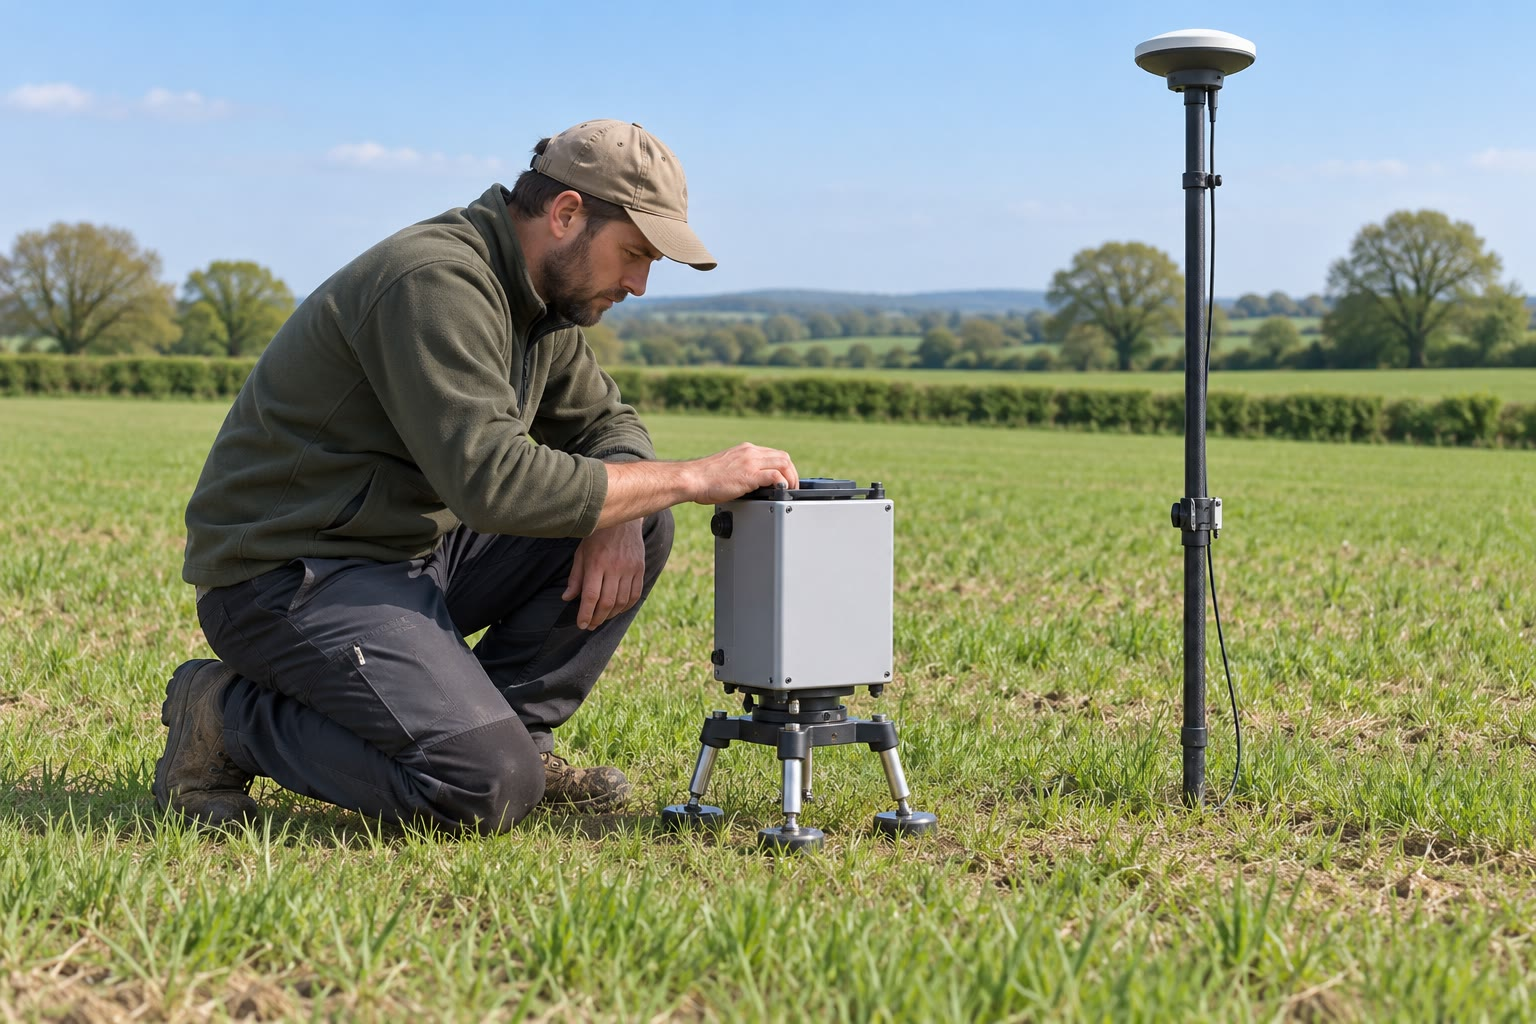
\includegraphics[width=\linewidth]{images/book3/ai/b1-gravity-survey.jpg}

{\scriptsize A field gravimeter on its tripod, with a satellite-positioning
antenna beside it (AI-generated illustration).}
\end{minipage}
\end{inthefield}

\section{Isostasy}

The compensation that Airy and Pratt imagined for the Himalaya is an instance of
a general state of the Earth's outer layers.

\begin{definition}[Isostasy; compensation depth]\label{def:b1:isostasy-gravity:isostasy}
A region is in \emph{isostasy}\index{isostasy}, or isostatic equilibrium, when
there exists a depth, the \emph{compensation depth}\index{compensation depth},
at which the pressure is the same at every point of the horizontal surface,
whatever the relief above. Below the compensation depth the rocks behave as a
fluid at rest; above it, the columns of \omterm{def:b1:layered-earth:layers}{crust} and \omterm{def:b1:layered-earth:layers}{mantle} float on them.
\end{definition}

\begin{proposition}[Equal masses above the compensation depth]\label{prop:b1:isostasy-gravity:equal-mass}
If gravity $g$ is the same along all the columns, a region is in \omterm{def:b1:isostasy-gravity:isostasy}{isostasy} with
\omterm{def:b1:isostasy-gravity:isostasy}{compensation depth} $z_c$ if and only if every vertical column of unit
cross-section, from the surface down to $z_c$, contains the same mass.
\end{proposition}

\begin{proof}
In each column the rocks are in hydrostatic equilibrium, so that
$\mathrm dp/\mathrm dz = \rho(z)\,g$, with the depth $z$ counted downwards. The
pressure at the surface is atmospheric, the same everywhere (and negligible).
Integrating from the surface $z_s$ of the column down to $z_c$ gives
\[
  p(z_c) = p_0 + g\int_{z_s}^{z_c}\rho(z)\,\mathrm dz ,
\]
where the integral is the mass of the column per unit area. The pressures at
$z_c$ are equal if and only if these masses are.
\end{proof}

Two simple ways of distributing the masses give the two classical models
(figure below).

\begin{proposition}[Airy isostasy]\label{prop:b1:isostasy-gravity:airy}
Let the \omterm{def:b1:layered-earth:layers}{crust} have a uniform density $\rho_c$ and a thickness $H$ where its
surface is at sea level, over a \omterm{def:b1:layered-earth:layers}{mantle} of density $\rho_m > \rho_c$. In isostatic
equilibrium:
\begin{enumerate}
  \item where the surface stands at a height $h$ above sea level, the \omterm{def:b1:layered-earth:layers}{crust} has
        a root of depth $r = h\,\rho_c/(\rho_m - \rho_c)$ below the normal \omterm{def:b1:layered-earth:layers}{crust},
        and a thickness $H + h + r$;
  \item where the surface lies at a depth $d$ below sea level, under water of
        density $\rho_w$, the \omterm{def:b1:layered-earth:layers}{crust} has an anti-root: its base is raised by
        $r' = d\,(\rho_c - \rho_w)/(\rho_m - \rho_c)$, and its thickness is
        $H - d - r'$.
\end{enumerate}
This is \emph{Airy isostasy}\index{Airy isostasy}: compensation by changes of
thickness at constant density.
\end{proposition}

\begin{proof}
Take the \omterm{def:b1:isostasy-gravity:isostasy}{compensation depth} just below the deepest root, and compare each
column with the normal one. (1) The high column has \omterm{def:b1:layered-earth:layers}{crust} in place of \omterm{def:b1:layered-earth:layers}{mantle}
over the depth $r$, and \omterm{def:b1:layered-earth:layers}{crust} over the height $h$ where the normal column has
nothing: equal masses require $\rho_c(h + r) = \rho_m r$, that is
$r(\rho_m - \rho_c) = \rho_c h$. (2) The low column has water in place of \omterm{def:b1:layered-earth:layers}{crust}
over the depth $d$, and \omterm{def:b1:layered-earth:layers}{mantle} in place of \omterm{def:b1:layered-earth:layers}{crust} over $r'$: equal masses require
$\rho_w d + \rho_m r' = \rho_c(d + r')$, that is $r'(\rho_m - \rho_c) =
d(\rho_c - \rho_w)$.
\end{proof}

\begin{proposition}[Pratt isostasy]\label{prop:b1:isostasy-gravity:pratt}
Let every column end at the same \omterm{def:b1:isostasy-gravity:isostasy}{compensation depth} $D$ below sea level, with a
uniform density in each column, $\rho_0$ where the surface is at sea level. In
isostatic equilibrium a column whose surface stands at a height $h$ has the
density
\[
  \rho(h) = \rho_0\,\frac{D}{D + h},
\]
and a column under a depth $d$ of water has the density
$\rho = (\rho_0 D - \rho_w d)/(D - d)$. This is \emph{Pratt
isostasy}\index{Pratt isostasy}: compensation by changes of density at constant
depth.
\end{proposition}

\begin{proof}
Equal masses above $D$: $\rho(h)(D + h) = \rho_0 D$ for the high column, and
$\rho_w d + \rho(D - d) = \rho_0 D$ for the low one.
\end{proof}

With $\rho_c = \qty{2700}{kg.m^{-3}}$ and $\rho_m = \qty{3300}{kg.m^{-3}}$, Airy's
root is $h\times2700/600 = 4.5\,h$: a range \qty{2}{km} high has a root of
\qty{9}{km}, a plateau \qty{4}{km} high one of \qty{18}{km}. In Pratt's model
with $D = \qty{100}{km}$ and $\rho_0 = \qty{2700}{kg.m^{-3}}$, the same two
columns have the densities 2647 and \qty{2596}{kg.m^{-3}}, two and four per cent
lighter. Both models balance the same masses; they differ in where the light
rock sits, and that is something seismology can see: Airy predicts a \omterm{def:b1:layered-earth:discontinuity}{Moho} that
deepens under the mountains, Pratt a flat one.

\begin{omfigure}
\begin{tikzpicture}[x=0.55cm, y=0.05cm, font=\scriptsize]
% columns computed in calc/ch11.py: Airy roots 9 and 18 km, Pratt densities 2647 and 2596 kg/m3;
% heights above sea level drawn five times larger than depths
\begin{scope}
  \node[font=\small] at (4.5,30) {(a) Airy};
  \fill[omLithGranite!45] (0,0) rectangle (3,-35);
  \fill[omLithGranite!45] (3,10) rectangle (6,-44);
  \fill[omLithGranite!45] (6,20) rectangle (9,-53);
  \fill[omLithPeridotite!45] (0,-35) rectangle (3,-60);
  \fill[omLithPeridotite!45] (3,-44) rectangle (6,-60);
  \fill[omLithPeridotite!45] (6,-53) rectangle (9,-60);
  \draw (0,-60) -- (0,0) -- (3,0) -- (3,10) -- (6,10) -- (6,20) -- (9,20) -- (9,-60);
  \draw (3,0) -- (3,-60) (6,10) -- (6,-60);
  \draw[thick] (0,-35) -- (3,-35) -- (3,-44) -- (6,-44) -- (6,-53) -- (9,-53);
  \draw[densely dashed] (-0.3,-60) -- (9.3,-60);
  \draw[black!50, densely dotted] (-0.3,0) -- (0,0);
  \node[anchor=east] at (-0.3,0) {sea level};
  \node[anchor=east] at (-0.3,-35) {35};
  \node[anchor=east] at (-0.3,-60) {60 km};
  \node at (1.5,-17) {2700}; \node at (4.5,-20) {2700}; \node at (7.5,-24) {2700};
  \node at (1.5,-50) {3300};
  \node[anchor=south] at (1.5,0) {$h = 0$};
  \node[anchor=south] at (4.5,10) {$h = 2$};
  \node[anchor=south] at (7.5,20) {$h = 4$};
  \draw[black!45, densely dotted] (3,-35) -- (9,-35);
  \node at (4.5,-39.5) {root 9};
  \node at (7.5,-44) {root 18};
\end{scope}
\begin{scope}[xshift=7.9cm]
  \node[font=\small] at (4.5,30) {(b) Pratt};
  \fill[omLithGranite!45] (0,0) rectangle (3,-100);
  \fill[omLithGranite!36] (3,10) rectangle (6,-100);
  \fill[omLithGranite!27] (6,20) rectangle (9,-100);
  \draw (0,-100) -- (0,0) -- (3,0) -- (3,10) -- (6,10) -- (6,20) -- (9,20) -- (9,-100);
  \draw (3,0) -- (3,-100) (6,10) -- (6,-100);
  \draw[densely dashed] (-0.3,-100) -- (9.3,-100);
  \draw[black!50, densely dotted] (-0.3,0) -- (0,0);
  \node[anchor=east] at (-0.3,0) {sea level};
  \node[anchor=east] at (-0.3,-100) {$D = 100$ km};
  \node at (1.5,-50) {2700}; \node at (4.5,-50) {2647}; \node at (7.5,-50) {2596};
  \node[anchor=south] at (1.5,0) {$h = 0$};
  \node[anchor=south] at (4.5,10) {$h = 2$};
  \node[anchor=south] at (7.5,20) {$h = 4$};
\end{scope}
\end{tikzpicture}

\par\smallskip{\small The two classical models of \omterm{def:b1:isostasy-gravity:isostasy}{isostasy}, for three columns
standing 0, 2 and \qty{4}{km} above sea level (heights exaggerated five times
against depths; densities in \unit{kg.m^{-3}}). (a) Airy: one crustal density,
a root 4.5 times the height. (b) Pratt: one \omterm{def:b1:isostasy-gravity:isostasy}{compensation depth}, lighter columns
under higher ground. Every column carries the same mass per unit area above the
dashed \omterm{def:b1:isostasy-gravity:isostasy}{compensation depth}.}
\label{fig:b1:isostasy-gravity:models}
\end{omfigure}

\omterm{def:b1:isostasy-gravity:isostasy}{Isostasy} is a statement about wide regions over long times. The \omterm{def:b1:layered-earth:lithosphere}{asthenosphere}
yields only to loads that persist for thousands of years, and the \omterm{def:b1:layered-earth:lithosphere}{lithosphere}
above it is stiff enough to spread a narrow load over a broad region by bending,
as a plank carries a weight: a single volcano need not be compensated beneath
itself; this flexure of the \omterm{def:b1:layered-earth:lithosphere}{lithosphere} is studied in Book 5. Under large
mountain ranges the \omterm{def:b1:layered-earth:layers}{crust} is far thicker than its continental average of about
\qty{30}{km}: Airy's picture, roots of light \omterm{def:b1:layered-earth:layers}{crust}, is the closer one for
mountain ranges. Pratt's, lighter rock at constant depth, explains the
mid-ocean ridges, which stand high over an upper \omterm{def:b1:layered-earth:layers}{mantle} made lighter by its
higher temperature.
% ledger: usgs:crust-thickness

\subsection*{The Earth's two levels}

\omterm{def:b1:isostasy-gravity:isostasy}{Isostasy} organises the relief of the whole planet. Its distribution is
summarised by one curve.

\begin{definition}[Hypsometric curve]\label{def:b1:isostasy-gravity:hypsometry}
The \emph{hypsometric curve}\index{hypsometric curve} of a planet gives, for
each fraction $f$ of its surface, the elevation $z(f)$ exceeded by exactly that
fraction. It is the cumulative distribution of elevation, read from the top.
\end{definition}

To draw it from a gridded elevation model, every grid cell must be weighted by
its area. On a grid of one degree in \omterm{def:b1:spherical-astronomy:geographic}{latitude} and \omterm{def:b1:spherical-astronomy:geographic}{longitude}, the cell between
the \omterm{def:b1:spherical-astronomy:geographic}{latitudes} $\varphi_1$ and $\varphi_2$ has the area
$R^2\,\Delta\lambda\,(\sin\varphi_2 - \sin\varphi_1)$, which shrinks towards the
poles; summed over all cells, the areas give $4\pi R^2$ exactly. Sorting the
cells by elevation and accumulating their areas gives the curve of the figure
below. It shows that \qty{70.9}{\percent} of the surface lies below sea level;
that the mean elevation of the land is about \qty{0.8}{km} and the mean depth
of the ocean about \qty{3.7}{km}; and that most of the surface belongs to one of
two flat steps, the continental platforms near sea level and the abyssal
floor between about 3.5 and \qty{6}{km} down, joined by a steep drop.
% computed in figdata/bachelor-1/hypsometry.py (fraction 0.709, land 793 m, ocean 3692 m); ledger: data:etopo1, wss:ocean-cover

A planet with a single kind of \omterm{def:b1:layered-earth:layers}{crust}, its relief raised and worn at random,
would have one level, with elevations scattered around it. The Earth has two,
because it has two kinds of \omterm{def:b1:layered-earth:layers}{crust} in isostatic equilibrium: the thick, light
continental \omterm{def:b1:layered-earth:layers}{crust} floats high, the thin, dense oceanic \omterm{def:b1:layered-earth:layers}{crust} low
(Book 2, grade 11). \Cref{exo:b1:isostasy-gravity:8} shows that Airy's model with one crustal
density cannot produce both levels with the observed crustal thicknesses.

\begin{omfigure}
\begin{tikzpicture}
\begin{axis}[omrecord, width=0.84\linewidth, height=6.4cm, xmin=0, xmax=100, ymin=-11, ymax=9,
  xlabel={fraction of the Earth's surface lying higher (\unit{\percent})},
  ylabel={elevation (km)}, xtick={0,10,...,100}, ytick={-10,-8,...,8},
  tick label style={font=\scriptsize}, label style={font=\small}, clip=true]
% computed in figdata/bachelor-1/hypsometry.py; ledger: data:etopo1
\addplot[name path=hyps, very thick, black] table[x=area_pc, y expr=\thisrow{elev}/1000] {figdata/out/bachelor-1-hypsometry-curve.dat};
\path[name path=sea] (axis cs:0,0) -- (axis cs:100,0);
\addplot[omSea!60] fill between[of=hyps and sea, soft clip={domain=29.1:100}];
\addplot[omHypsLandC!80] fill between[of=hyps and sea, soft clip={domain=0:29.1}];
\draw[black!60, densely dotted] (axis cs:0,0) -- (axis cs:100,0);
\draw[black!60, densely dashed] (axis cs:29.1,-11) -- (axis cs:29.1,9);
\draw[omSea!60!black, densely dashed] (axis cs:29.1,-3.692) -- (axis cs:100,-3.692);
\draw[omHypsLandF, densely dashed] (axis cs:0,0.793) -- (axis cs:29.1,0.793);
\node[font=\scriptsize, anchor=south east] at (axis cs:99,0.1) {sea level};
\node[font=\scriptsize, anchor=south, align=center] at (axis cs:18,1.0) {mean land\\elevation \qty{0.79}{km}};
\node[font=\scriptsize, anchor=north west, align=left] at (axis cs:31,-3.9) {mean ocean\\depth \qty{3.69}{km}};
\node[font=\scriptsize, anchor=north west, align=left] at (axis cs:30.5,6.5) {land: \qty{29.1}{\percent}\\of the surface};
\node[font=\scriptsize, anchor=north, align=center] at (axis cs:17,-0.5) {continental\\platform};
\node[font=\scriptsize] at (axis cs:62,-5.2) {abyssal floor};
\end{axis}
\end{tikzpicture}

\par\smallskip{\small The Earth's \omterm{def:b1:isostasy-gravity:hypsometry}{hypsometric curve}, from the ETOPO1 global
relief model at one degree, each cell weighted by its area (over Antarctica and
Greenland, the top of the ice). The two nearly flat stretches of the curve are
the continental platforms near sea level and the deep ocean floor.}
\label{fig:b1:isostasy-gravity:hypsometry}
\end{omfigure}

\section{Gravity anomalies}

\subsection*{Two corrections}

A gravimeter on a hill is farther from the Earth's centre than one at sea level,
and stands on a layer of rock that the other does not have. Both effects are
computed before the measurement is compared with \omterm{def:b1:isostasy-gravity:normal-gravity}{normal gravity}.

\begin{proposition}[Free-air gradient]\label{prop:b1:isostasy-gravity:free-air}
Outside a spherical Earth of radius $R$, gravity decreases with height $h$ at
the rate
\[
  \frac{\mathrm dg}{\mathrm dh} = -\frac{2g}{R}\,;
\]
at the surface, $2g/R \approx \qty{3.08e-6}{s^{-2}}$, about
\qty{0.308}{\milli\gal} per metre.
\end{proposition}

\begin{proof}
$g(r) = GM/r^2$, so $\mathrm dg/\mathrm dr = -2GM/r^3 = -2g(r)/r$; at $r = R$,
with $g = \qty{9.820}{m.s^{-2}}$ and $R = \qty{6371}{km}$, $2g/R =
\qty{3.083e-6}{s^{-2}}$.
\end{proof}
% ledger: earth:gmean, earth:Rmean

The flattening and the rotation change the gradient slightly; the value used in
practice is \qty{0.3086}{\milli\gal.m^{-1}}.
% ledger: usgs73:reduction

\begin{proposition}[Bouguer slab]\label{prop:b1:isostasy-gravity:slab}
An infinite horizontal slab of thickness $h$ and uniform density $\rho$ attracts
a point outside it with the vertical acceleration
\[
  g_B = 2\pi G\rho h ,
\]
whatever the distance from the point to the slab. Numerically $2\pi G =
\qty{0.0419}{\milli\gal}$ per metre of thickness per \qty{1000}{kg.m^{-3}} of
density.
\end{proposition}

\begin{proof}
Put the point at the origin and cut the slab into thin rings coaxial with the
vertical through it. A ring at the distance $z$ below the point, of radius
$s$, width $\mathrm ds$ and thickness $\mathrm dz$, has the mass
$\rho\,2\pi s\,\mathrm ds\,\mathrm dz$, all at the distance $\sqrt{s^2 + z^2}$;
by symmetry its attraction is vertical, equal to the attraction of each
element times the cosine $z/\sqrt{s^2+z^2}$ of its angle with the vertical:
\[
  \mathrm dg = G\,\frac{\rho\,2\pi s\,\mathrm ds\,\mathrm dz}{s^2 + z^2}\,
  \frac{z}{\sqrt{s^2 + z^2}} .
\]
For one layer, $\int_0^\infty s\,(s^2 + z^2)^{-3/2}\,\mathrm ds =
\bigl[-(s^2 + z^2)^{-1/2}\bigr]_0^\infty = 1/z$, so the layer attracts with
$2\pi G\rho\,\mathrm dz$, independently of $z$. Adding the layers over the
thickness $h$ gives $2\pi G\rho h$. With $G = \qty{6.674e-11}{m^3.kg^{-1}.s^{-2}}$,
$2\pi G\times\qty{1000}{kg.m^{-3}}\times\qty{1}{m} = \qty{4.19e-7}{m.s^{-2}} =
\qty{0.0419}{\milli\gal}$.
\end{proof}
% ledger: const:G

\begin{definition}[Gravity anomalies]\label{def:b1:isostasy-gravity:anomalies}
Let $g$ be the gravity measured at a station of \omterm{def:b1:spherical-astronomy:geographic}{latitude} $\varphi$ and height $h$
above sea level.
\begin{itemize}
  \item A \emph{gravity anomaly}\index{gravity anomaly} is the difference
        between the measured gravity, corrected to a common level, and the
        \omterm{def:b1:isostasy-gravity:normal-gravity}{normal gravity} at the same \omterm{def:b1:spherical-astronomy:geographic}{latitude}.
  \item The \emph{free-air correction}\index{free-air correction} is
        $+\qty{0.3086}{\milli\gal.m^{-1}}\times h$: it adds back the decrease
        of gravity with height. The \emph{free-air
        anomaly}\index{free-air anomaly} is
        $\Delta g_{\mathrm{FA}} = g + 0.3086\,h - \gamma(\varphi)$.
  \item The \emph{Bouguer correction}\index{Bouguer correction} is $-2\pi G\rho h$:
        it removes the attraction of the rock between the station and sea
        level, treated as a slab of density $\rho$, conventionally
        \qty{2670}{kg.m^{-3}}, which gives \qty{0.112}{\milli\gal} per metre.
        The \emph{Bouguer anomaly}\index{Bouguer anomaly} is
        $\Delta g_{\mathrm B} = \Delta g_{\mathrm{FA}} - 2\pi G\rho h$.
\end{itemize}
\end{definition}
% ledger: usgs73:reduction, swisstopo:bouguer-map

The slab is a crude model of the ground around a station in rough country:
valleys below the station are counted as rock that is not there, hills above
it pull upwards and are not counted at all. A third reduction, the terrain
correction, computed from a \omterm{def:b1:geological-maps:dem}{digital elevation model}, removes both errors. At
sea the \omterm{def:b1:isostasy-gravity:anomalies}{free-air correction} vanishes, and the Bouguer reduction replaces the
water by rock.

\begin{method}[Reducing a gravity reading]\label{met:b1:isostasy-gravity:reduction}
\begin{enumerate}
  \item Compute the \omterm{def:b1:isostasy-gravity:normal-gravity}{normal gravity} $\gamma(\varphi)$ at the station's \omterm{def:b1:spherical-astronomy:geographic}{latitude}.
  \item Add the \omterm{def:b1:isostasy-gravity:anomalies}{free-air correction} $0.3086\,h$ (in \unit{\milli\gal}, with $h$
        in metres) to the measured gravity and subtract $\gamma$: this is the
        \omterm{def:b1:isostasy-gravity:anomalies}{free-air anomaly}.
  \item Subtract the \omterm{def:b1:isostasy-gravity:anomalies}{Bouguer correction} $0.0419\times(\rho/1000)\times h$, that is
        $0.112\,h$ for the standard density: this is the \omterm{def:b1:isostasy-gravity:anomalies}{Bouguer anomaly}.
  \item Work in milligals throughout, and keep the measured and \omterm{def:b1:isostasy-gravity:normal-gravity}{normal gravity}
        to seven significant figures: the anomaly is a small difference of two
        large numbers.
\end{enumerate}
\end{method}

\begin{example}[A station in the hills]\label{ex:b1:isostasy-gravity:reduction}
At a station at \omterm{def:b1:spherical-astronomy:geographic}{latitude} \ang{45} and \qty{1200}{m} above sea level, the
gravimeter gives \qty{9.802597}{m.s^{-2}}. \omterm{def:b1:isostasy-gravity:normal-gravity}{Normal gravity} there is
\qty{9.806200}{m.s^{-2}}; the measured value is lower by \qty{360.3}{\milli\gal}.
The \omterm{def:b1:isostasy-gravity:anomalies}{free-air correction} is $0.3086\times1200 = \qty{370.3}{\milli\gal}$, so
$\Delta g_{\mathrm{FA}} = -360.3 + 370.3 = \qty{+10.0}{\milli\gal}$. The \omterm{def:b1:isostasy-gravity:anomalies}{Bouguer
correction} is $0.112\times1200 = \qty{134.4}{\milli\gal}$, so $\Delta g_{\mathrm B}
= \qty{-124.4}{\milli\gal}$: there is less mass below this station than below a
station at sea level, once the rock above sea level is removed.
\end{example}

\subsection*{What the anomalies say about compensation}

\begin{proposition}[Anomalies over broad relief]\label{prop:b1:isostasy-gravity:broad}
Consider a plateau of height $h$ and density $\rho_c$, much wider than its
\omterm{def:b1:isostasy-gravity:isostasy}{compensation depth}, and a station near its centre. Take the Bouguer density
equal to $\rho_c$.
\begin{enumerate}
  \item If the plateau is not compensated, $\Delta g_{\mathrm{FA}} \approx
        2\pi G\rho_c h$ and $\Delta g_{\mathrm B} \approx 0$.
  \item If it is in isostatic equilibrium, whatever the distribution of the
        compensating masses, $\Delta g_{\mathrm{FA}} \approx 0$ and
        $\Delta g_{\mathrm B} \approx -2\pi G\rho_c h$.
\end{enumerate}
\end{proposition}

\begin{proof}
\omterm{def:b1:isostasy-gravity:normal-gravity}{Normal gravity} at the station's height is $\gamma - 0.3086\,h$, so the \omterm{def:b1:isostasy-gravity:anomalies}{free-air
anomaly} is the attraction of the masses that differ from those of a normal
column. Near the centre of a wide plateau each layer of these anomalous masses
acts as an infinite slab, and by \cref{prop:b1:isostasy-gravity:slab} a slab of
density contrast $\Delta\rho$ and thickness $t$ attracts with $2\pi G\Delta\rho
t$ wherever it lies. The total is $2\pi G$ times the anomalous mass per unit
area. (1) Without compensation that mass is $\rho_c h$. (2) In \omterm{def:b1:isostasy-gravity:isostasy}{isostasy} it is
zero by \cref{prop:b1:isostasy-gravity:equal-mass}. In both cases the \omterm{def:b1:isostasy-gravity:anomalies}{Bouguer
correction} subtracts $2\pi G\rho_c h$.
\end{proof}

For Airy compensation the \omterm{def:b1:isostasy-gravity:anomalies}{Bouguer anomaly} of the second case is also
$-2\pi G(\rho_m - \rho_c)r$, the attraction of the missing mass of the root,
since $(\rho_m - \rho_c)r = \rho_c h$. Free-air anomalies near zero over wide
regions are thus the signature of \omterm{def:b1:isostasy-gravity:isostasy}{isostasy}, and Bouguer anomalies that follow
the relief in mirror image measure the compensating masses: the Bouguer
anomalies are regionally negative all along the Alps, and over the mid-ocean
ridges, high as they are, the \omterm{def:b1:isostasy-gravity:anomalies}{free-air anomaly} is small. Over the oceans the
\omterm{def:b1:isostasy-gravity:anomalies}{Bouguer anomaly} is positive: replacing the water by rock adds mass above a
column that has none missing.
% ledger: swisstopo:bouguer-map

Near the edges of the relief the slab approximation fails, because the
topography is close to the station and the root far below it. The figure below
gives the exact attraction of a model range \qty{200}{km} wide and \qty{2}{km}
high. Without compensation, the \omterm{def:b1:isostasy-gravity:anomalies}{free-air anomaly} is
\qty{+225}{\milli\gal} at the centre, close to the slab value of
\qty{226}{\milli\gal}; with an Airy root of \qty{9}{km}, the centre \omterm{def:b1:isostasy-gravity:anomalies}{free-air
anomaly} falls to \qty{+55}{\milli\gal}, not zero, because a range only
\qty{200}{km} wide does not look infinite from \qty{40}{km} above its root, and
the \omterm{def:b1:isostasy-gravity:anomalies}{free-air anomaly} turns sharply negative just beyond each edge, where the
station sees the root but not the mountain.
% computed in figdata/bachelor-1/gravity_profiles.py (centre values 225.0, -1.4, 55.2, -171.2 mGal)

\begin{omfigure}
\begin{tikzpicture}
\begin{axis}[omrecord, name=anom, width=0.86\linewidth, height=6.2cm, xmin=-300, xmax=300, ymin=-310, ymax=250,
  ylabel={anomaly (\unit{\milli\gal})}, xticklabels={}, ytick={-200,-100,0,100,200},
  tick label style={font=\scriptsize}, label style={font=\small},
  legend style={font=\scriptsize, at={(0.01,0.01)}, anchor=south west, draw=none, fill=white, fill opacity=0.85, text opacity=1},
  legend cell align=left, legend columns=2]
% computed in figdata/bachelor-1/gravity_profiles.py
\addplot[very thick, red!75!black] table[x=x, y=fa_unc] {figdata/out/bachelor-1-gravity_profiles-profiles.dat};
\addlegendentry{free-air, uncompensated}
\addplot[thick, red!75!black, densely dashed] table[x=x, y=bg_unc] {figdata/out/bachelor-1-gravity_profiles-profiles.dat};
\addlegendentry{Bouguer, uncompensated}
\addplot[very thick, blue!70!black] table[x=x, y=fa_airy] {figdata/out/bachelor-1-gravity_profiles-profiles.dat};
\addlegendentry{free-air, Airy root}
\addplot[thick, blue!70!black, densely dashed] table[x=x, y=bg_airy] {figdata/out/bachelor-1-gravity_profiles-profiles.dat};
\addlegendentry{Bouguer, Airy root}
\draw[black!50, densely dotted] (axis cs:-300,0) -- (axis cs:300,0);
\end{axis}
\begin{axis}[at={(anom.south west)}, anchor=north west, yshift=-0.25cm, width=0.86\linewidth, height=3.6cm,
  xmin=-300, xmax=300, ymin=-50, ymax=5, axis background/.style={fill=white},
  xlabel={distance from the centre of the range (km)}, ylabel={depth (km)},
  ytick={0,-35,-44}, yticklabels={0,35,44}, tick label style={font=\scriptsize}, label style={font=\small}]
\fill[omLithPeridotite!45] (axis cs:-300,-50) rectangle (axis cs:300,-35);
\fill[omLithGranite!45] (axis cs:-300,-35) rectangle (axis cs:300,0);
\fill[omLithGranite!45] (axis cs:-100,0) rectangle (axis cs:100,2);
\fill[omLithGranite!45, pattern color=blue!60!black, postaction={pattern=north east lines, pattern color=blue!50!black}] (axis cs:-100,-35) rectangle (axis cs:100,-44);
\draw (axis cs:-300,0) -- (axis cs:-100,0) -- (axis cs:-100,2) -- (axis cs:100,2) -- (axis cs:100,0) -- (axis cs:300,0);
\draw[thick] (axis cs:-300,-35) -- (axis cs:300,-35);
\draw[thick, blue!60!black] (axis cs:-100,-35) -- (axis cs:-100,-44) -- (axis cs:100,-44) -- (axis cs:100,-35);
\node[font=\scriptsize] at (axis cs:-200,-17) {crust 2700};
\node[font=\scriptsize] at (axis cs:-200,-43) {mantle 3300};
\node[font=\scriptsize, fill=white, inner sep=1pt, anchor=west] at (axis cs:105,-40) {Airy root (second model)};
\node[font=\scriptsize, anchor=south] at (axis cs:0,2) {range, \qty{2}{km} high};
\end{axis}
\end{tikzpicture}

\par\smallskip{\small Top: free-air and Bouguer anomalies across a model range
\qty{200}{km} wide and \qty{2}{km} high, computed exactly for two-dimensional
bodies, with stations on the ground surface (no terrain correction). Bottom:
the model (vertical scale exaggerated less than twice); the root exists only in
the compensated case. Uncompensated, the \omterm{def:b1:isostasy-gravity:anomalies}{free-air anomaly} follows the relief and
the \omterm{def:b1:isostasy-gravity:anomalies}{Bouguer anomaly} is nearly zero; compensated, the \omterm{def:b1:isostasy-gravity:anomalies}{free-air anomaly} is small
at the centre with sharp edge effects, and the \omterm{def:b1:isostasy-gravity:anomalies}{Bouguer anomaly} is a broad
trough.}
\label{fig:b1:isostasy-gravity:profiles}
\end{omfigure}

\begin{method}[Testing a region for isostasy]\label{met:b1:isostasy-gravity:test}
\begin{enumerate}
  \item Average the \omterm{def:b1:isostasy-gravity:anomalies}{free-air anomaly} over an area several times wider than the
        \omterm{def:b1:layered-earth:layers}{crust} is thick, away from the edges of the relief.
  \item If it is near zero, the region is compensated; if it approaches
        $2\pi G\rho_c$ times the mean height, it is not.
  \item The ratio $-\Delta g_{\mathrm B}/(2\pi G\rho_c h)$ gives the fraction of
        the relief that is compensated.
  \item Seismic or other evidence on the depth of the \omterm{def:b1:layered-earth:discontinuity}{Moho} tells Airy's
        compensation from Pratt's: broad gravity alone cannot, since both put
        the same mass deficit below the relief.
\end{enumerate}
\end{method}

\begin{history}[Gravity at sea]
\begin{minipage}[t]{0.58\linewidth}\vspace{0pt}
A pendulum measures gravity through its period, but on a ship the waves shake
it far more than any anomaly. In the 1920s the Dutch geodesist Felix Vening
Meinesz found the way round: two pendulums swinging in opposite phase in the
same frame feel the same horizontal accelerations of the ship, and their
difference cancels them. From 1923 he carried his apparatus on submarines of
the Dutch navy, where, submerged, it was spared the worst of the waves, first
on a voyage to the East Indies and then in surveys of their seas. Along the
deep-sea trenches of the archipelago he found long belts of strongly negative
isostatic anomalies, and then found them along other trenches: he could explain
them only by a \omterm{def:b1:layered-earth:layers}{crust} held down there by outside forces, out of isostatic
equilibrium.
% ledger: egs:vening-meinesz
\end{minipage}\hfill
\begin{minipage}[t]{0.38\linewidth}\vspace{0pt}
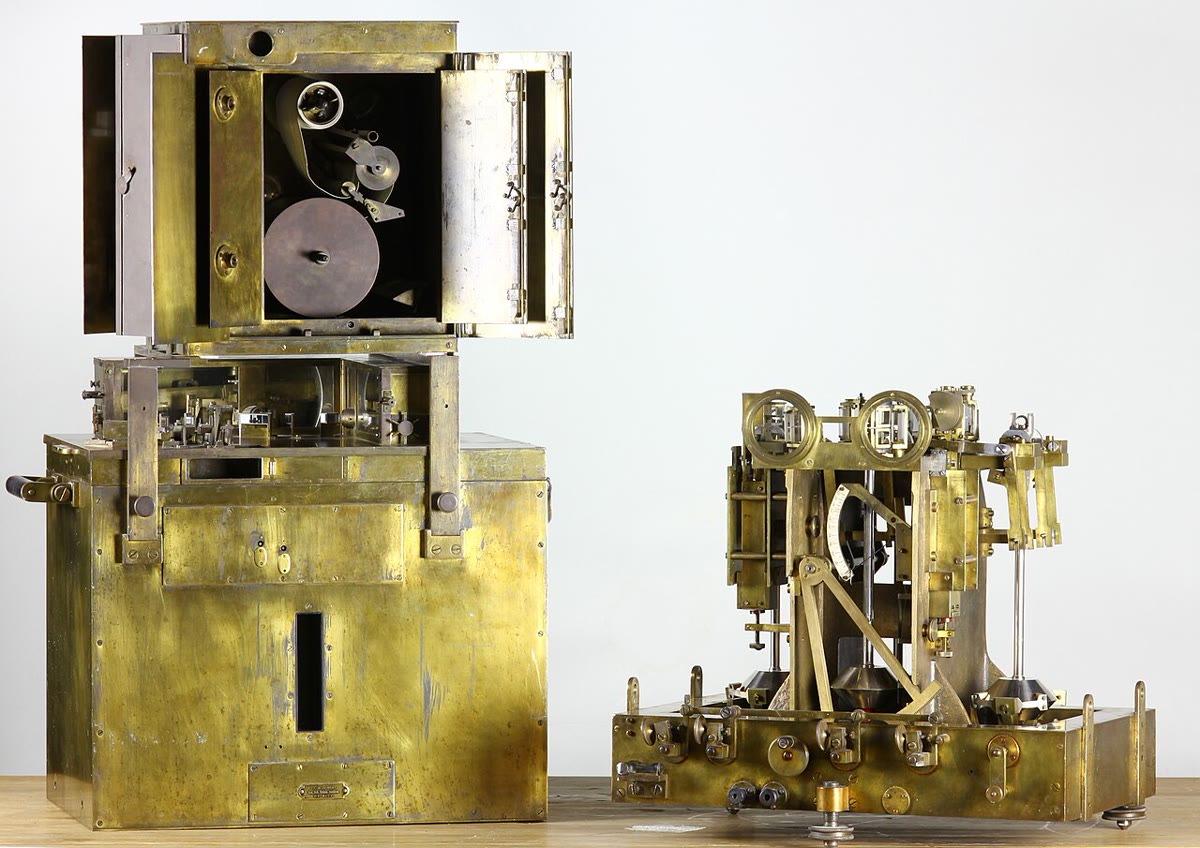
\includegraphics[width=\linewidth]{images/book3/b1-vening-meinesz.jpg}

{\scriptsize A Vening Meinesz pendulum apparatus (right) and its case with
the recording unit (Broodt, CC BY-SA 4.0).}
\end{minipage}
\end{history}

\section{The geoid}

The sea surface at rest is a surface of constant gravity potential: if it were
not, water would flow along it. It is the natural reference for heights, and
the surface the old plumb lines were perpendicular to.

\begin{definition}[Geoid; geoid height]\label{def:b1:isostasy-gravity:geoid}
The \emph{geoid}\index{geoid} is the equipotential surface of the Earth's
gravity (gravitation plus the centrifugal effect of rotation) that coincides
with the mean sea surface over the open oceans, at rest, and is continued
beneath the continents. The \emph{geoid height}\index{geoid height} $N$ at a
point is the height of the geoid above the reference ellipsoid, counted
negative where the geoid lies below it.
\end{definition}

Heights above sea level on maps are heights above the \omterm{def:b1:isostasy-gravity:geoid}{geoid}; the heights given
by satellite positioning are heights above the ellipsoid; the two differ by
$N$. The \omterm{def:b1:isostasy-gravity:geoid}{geoid} departs from the ellipsoid by \qty{+85}{m} near Iceland and
\qty{-106}{m} off southern India, less than \qty{200}{m} in all, while the relief
of the solid surface spans about \qty{20}{km}: the \omterm{def:b1:isostasy-gravity:geoid}{geoid} is a far smoother
surface than the ground.
% ledger: nasa:geoid-range, earth:topo

\begin{proposition}[Geoid height and potential anomaly]\label{prop:b1:isostasy-gravity:bruns}
Let $\Phi$ be the Earth's gravity potential and $\Phi_n$ the normal potential,
that of the model Earth whose surface, the reference ellipsoid, has the same
potential $\Phi_0$ as the \omterm{def:b1:isostasy-gravity:geoid}{geoid}, both counted with the sign of physics (the
potential increases upwards and $g = -\nabla\Phi$). Let $T = \Phi - \Phi_n$ be the
potential anomaly at the \omterm{def:b1:isostasy-gravity:geoid}{geoid}. To first order,
\[
  N = -\frac{T}{\gamma} .
\]
Geodesists, who count the potential with the opposite sign, write the same
result $N = T/\gamma$, Bruns' formula.
\end{proposition}

\begin{proof}
Let $Q$ be a point of the ellipsoid and $P$ the point of the \omterm{def:b1:isostasy-gravity:geoid}{geoid} on the
normal through $Q$, at the height $N$. The normal potential increases upwards
at the rate $\gamma$, so $\Phi_n(P) \approx \Phi_n(Q) + \gamma N = \Phi_0 +
\gamma N$. Since $P$ is on the \omterm{def:b1:isostasy-gravity:geoid}{geoid}, $\Phi(P) = \Phi_0$, that is
$\Phi_n(P) + T = \Phi_0$. Hence $\Phi_0 + \gamma N + T = \Phi_0$ and $N =
-T/\gamma$.
\end{proof}

An excess of mass below a point makes the potential there more negative, so
$T < 0$ and $N > 0$: the \omterm{def:b1:isostasy-gravity:geoid}{geoid} bulges up over excess mass and sinks over a
deficit. The \qty{85}{m} of the high near Iceland correspond to a potential
anomaly of $-\qty{85}{m}\times\qty{9.8}{m.s^{-2}} \approx \qty{-830}{J.kg^{-1}}$.
Because the potential falls off as $1/r$ while the attraction falls off as $1/r^2$,
the \omterm{def:b1:isostasy-gravity:geoid}{geoid} is dominated by large, deep masses, and the gravity anomalies by
shallow ones. A compensated mountain range raises the \omterm{def:b1:isostasy-gravity:geoid}{geoid} only slightly,
because its mass excess and its root's deficit nearly cancel; an
uncompensated load raises it much more.

\begin{omfigure}
\begin{tikzpicture}[x=1.15cm, y=1.3cm, font=\scriptsize, >={Stealth[length=4pt]}]
% schematic, not to scale
\fill[omSea!35] (0,0.05) .. controls (1.5,0.25) and (2.5,0.35) .. (3.6,0.45) -- (3.6,-1.2) -- (0,-1.2) -- cycle;
\fill[omLithGranite!40] (3.6,0.45) .. controls (4.5,1.4) and (5.4,1.9) .. (6.4,1.7) .. controls (7.4,1.5) and (8.2,1.2) .. (9,1.0) -- (9,-1.2) -- (3.6,-1.2) -- cycle;
\fill[omLithGabbro!35] (0,-0.7) .. controls (1.2,-0.9) and (2.4,-0.6) .. (3.6,-0.2) -- (3.6,-1.2) -- (0,-1.2) -- cycle;
\draw[thick, blue!70!black] (0,0.05) .. controls (1.5,0.25) and (2.5,0.35) .. (3.6,0.45) .. controls (5,0.75) and (7,0.75) .. (9,0.55);
\draw[thick, black, densely dashed] (0,-0.25) .. controls (3,0.05) and (6,0.15) .. (9,0.1);
\draw (3.6,0.45) .. controls (4.5,1.4) and (5.4,1.9) .. (6.4,1.7) .. controls (7.4,1.5) and (8.2,1.2) .. (9,1.0);
\node[anchor=west, blue!70!black] at (9.05,0.6) {geoid};
\node[anchor=west] at (9.05,0.1) {ellipsoid};
\node[anchor=west] at (9.05,1.0) {ground};
\node at (1.4,-0.3) {ocean};
\node at (1.6,-1.0) {sea floor};
% heights (curve ordinates computed from the Bezier segments)
\draw[<->] (6.6,0.107) -- (6.6,0.688); \node[anchor=east] at (6.57,0.40) {$N$};
\draw[<->] (7.2,0.674) -- (7.2,1.512); \node[anchor=west] at (7.23,1.09) {$H$};
\draw[<->] (8.2,0.110) -- (8.2,1.224); \node[anchor=east] at (8.17,0.95) {$h_e$};
% the vertical (perpendicular to the geoid) and the ellipsoid normal at x = 2.4 (angle exaggerated)
\draw[->, thick, blue!70!black] (2.4,0.335) -- (2.0,1.3);
\draw[->, thick, black] (2.4,0.335) -- (2.33,1.3);
\node[anchor=south east, blue!70!black] at (2.05,1.3) {vertical (plumb line)};
\node[anchor=south west] at (2.3,1.3) {ellipsoid normal};
\end{tikzpicture}

\par\smallskip{\small The \omterm{def:b1:isostasy-gravity:geoid}{geoid} (blue), the reference ellipsoid (dashed) and the
ground (schematic; departures enormously exaggerated). Over the ocean the \omterm{def:b1:isostasy-gravity:geoid}{geoid}
is the sea surface at rest; under the land it is continued as an equipotential.
The height $H$ on a map is measured from the \omterm{def:b1:isostasy-gravity:geoid}{geoid}, the height $h_e$ given by
satellite positioning from the ellipsoid, and $h_e = H + N$. A plumb line is
perpendicular to the \omterm{def:b1:isostasy-gravity:geoid}{geoid}, not to the ellipsoid: the angle between them
(exaggerated here) is the deflection of the vertical that troubled the
surveyors of India.}
\label{fig:b1:isostasy-gravity:geoid}
\end{omfigure}

The deflections are small: the whole discrepancy that troubled the surveyors
of India was about five seconds of arc. Over the oceans the \omterm{def:b1:isostasy-gravity:geoid}{geoid} is visible.
Since 1978, radar altimeters on satellites have timed microwave pulses
reflected from the sea surface to measure its height. Once tides, waves and
currents are averaged away, the sea surface stands higher over seamounts and
ridges and lower over trenches and abyssal plains, and these bumps (\cref{exo:b1:isostasy-gravity:11}
estimates one) map the topography of the deep ocean floor where no ship has
sounded. The satellite GOCE, from 2009 to 2013, flew at about \qty{260}{km}
and measured the gravity field from orbit, aiming at the \omterm{def:b1:isostasy-gravity:geoid}{geoid} to 1 to
\qty{2}{cm} and the gravity anomalies to about \qty{1}{\milli\gal}, with a
resolution better than \qty{100}{km}.
% ledger: pratt:himalaya, jpl:seasat, esa:goce

\subsection*{Isostasy in motion}

\omterm{def:b1:isostasy-gravity:isostasy}{Isostasy} is reached by flow, and flow takes time. At the peak of the last
glaciation, about \num{20000} years ago, an ice sheet about \qty{3}{km} thick
covered Scandinavia.
Ice is about nine tenths as dense as water, so with a \omterm{def:b1:layered-earth:layers}{mantle} of
\qty{3300}{kg.m^{-3}}, the full isostatic depression under such a sheet is
$\qty{3000}{m}\times900/3300 \approx \qty{820}{m}$. The ice has gone, and the
land is still rising: satellite positioning measures up to about
\qty{10}{mm.yr^{-1}} of uplift in northern Sweden, west of the Gulf of Bothnia,
today. The
rate at which a depression relaxes measures the viscosity of the \omterm{def:b1:layered-earth:layers}{mantle} below,
the subject of Book 5; \cref{exo:b1:isostasy-gravity:12} shows how.
% ledger: kierulf:fennoscandia, usgs:ice-density

\section{Exercises}

\begin{exercise}[$\star$]\label{exo:b1:isostasy-gravity:1}
(a) Convert a \omterm{def:b1:isostasy-gravity:anomalies}{Bouguer anomaly} of \qty{-150}{\milli\gal} to \unit{m.s^{-2}},
and express it as a fraction of $g = \qty{9.81}{m.s^{-2}}$. (b) The same for
\qty{1}{\milli\gal}, the precision aimed at for the gravity anomalies from
GOCE, and for \qty{1}{\micro\gal}.
% ledger: esa:goce, nist:gal
\end{exercise}

\begin{exercise}[$\star$]\label{exo:b1:isostasy-gravity:2}
(a) Compute \omterm{def:b1:isostasy-gravity:normal-gravity}{normal gravity} at the equator, at \ang{45} and at the poles with
the formula of the chapter. (b) Give the equator-to-pole difference in
milligals. (c) The centrifugal acceleration at the equator is
\qty{3392}{\milli\gal}. What fraction of the difference does the rotation
explain directly?
% ledger: moritz:grs80
\end{exercise}

\begin{exercise}[$\star$]\label{exo:b1:isostasy-gravity:3}
A plateau stands \qty{3}{km} above sea level. With a \omterm{def:b1:layered-earth:layers}{crust} of density
\qty{2800}{kg.m^{-3}} and a \omterm{def:b1:layered-earth:layers}{mantle} of \qty{3300}{kg.m^{-3}}, compute its Airy root
and the thickening of its \omterm{def:b1:layered-earth:layers}{crust}.
\end{exercise}

\begin{exercise}[$\star$]\label{exo:b1:isostasy-gravity:4}
(a) By how much must a gravimeter be raised for its reading to fall by
\qty{1}{\milli\gal}? Use \qty{0.3086}{\milli\gal.m^{-1}}. (b) A survey aims at
anomalies to \qty{0.01}{\milli\gal}. To what accuracy must the station heights
be known?
\end{exercise}

\begin{exercise}[$\star\star$]\label{exo:b1:isostasy-gravity:5}
In Pratt's model with $D = \qty{100}{km}$ and $\rho_0 = \qty{2700}{kg.m^{-3}}$,
(a) compute the density of the columns that stand 1, 3 and \qty{5}{km} high;
(b) compute the density of a column under \qty{4}{km} of sea water of density
\qty{1030}{kg.m^{-3}}. (c) Why is Pratt's model better suited to the ocean
floor than to the continents?
\end{exercise}

\begin{exercise}[$\star\star$]\label{exo:b1:isostasy-gravity:6}
Two stations lie at \omterm{def:b1:spherical-astronomy:geographic}{latitude} \ang{48}, where \omterm{def:b1:isostasy-gravity:normal-gravity}{normal gravity} is
\qty{9.808911}{m.s^{-2}}. Station 1, \qty{350}{m} above sea level, reads
\qty{9.807751}{m.s^{-2}}; station 2, at \qty{1850}{m}, reads
\qty{9.803552}{m.s^{-2}}. (a) Compute the free-air and Bouguer anomalies of
both, with the standard Bouguer density. (b) What do the anomalies of station 2
suggest about the mountains around it?
\end{exercise}

\begin{exercise}[$\star\star$]\label{exo:b1:isostasy-gravity:7}
(a) Following the proof of \cref{prop:b1:isostasy-gravity:slab}, show that a
horizontal disc of radius $a$, thickness $h$ and density $\rho$ attracts a point
on its axis, at a distance $z \gg h$ above it, with $2\pi G\rho h\,\bigl(1 -
z/\sqrt{z^2 + a^2}\bigr)$. (b) What radius gives \qty{90}{\percent} of the slab
value at $z = \qty{1}{km}$? (c) What does this say about the area of terrain
that matters for the \omterm{def:b1:isostasy-gravity:anomalies}{Bouguer correction}?
\end{exercise}

\begin{exercise}[$\star\star$]\label{exo:b1:isostasy-gravity:8}
In Airy's model with a \omterm{def:b1:layered-earth:layers}{crust} of \qty{2800}{kg.m^{-3}}, \qty{35}{km} thick at sea
level, over a \omterm{def:b1:layered-earth:layers}{mantle} of \qty{3300}{kg.m^{-3}}, (a) compute the anti-root and the
crustal thickness under \qty{4}{km} of sea water of density \qty{1030}{kg.m^{-3}}.
(b) The oceanic \omterm{def:b1:layered-earth:layers}{crust} is in fact about \qty{5}{km} thick. What does the
difference show? % ledger: usgs:crust-thickness
\end{exercise}

\begin{exercise}[$\star\star$]\label{exo:b1:isostasy-gravity:9}
In the account of the opening, the discrepancy in the difference of \omterm{def:b1:spherical-astronomy:geographic}{latitude}
between Kaliana and Kalianpur was \qty{5.236}{''}, while the attraction of the
Himalaya computed by Pratt should have produced \qty{15.885}{''}. (a) Convert
both angles to radians. (b) A horizontal acceleration $a_h$ tilts a plumb line by
the angle $a_h/g$. What difference of horizontal attraction between the two
stations does each angle correspond to, in milligals, with
$g = \qty{9.79}{m.s^{-2}}$? (c) What fraction of the attraction of the visible
mountains did the compensation cancel?
% ledger: pratt:himalaya
\end{exercise}

\begin{exercise}[$\star\star\star$]\label{exo:b1:isostasy-gravity:10}
A salt dome is modelled as a sphere of radius \qty{2}{km}, its centre at
\qty{4}{km} depth, with a density \qty{200}{kg.m^{-3}} lower than the rocks
around it. (a) Show that a buried sphere of anomalous mass $M$ at depth $z$
gives, at the horizontal distance $x$, the anomaly $GMz/(x^2 + z^2)^{3/2}$.
(b) Compute the anomaly above its centre. (c) At what distance has it fallen
to half its peak value? (d) How could the depth of a sphere be read from a
measured profile?
\end{exercise}

\begin{exercise}[$\star\star\star$]\label{exo:b1:isostasy-gravity:11}
A seamount is a cone \qty{3}{km} high with a base of radius \qty{15}{km}
standing on a sea floor \qty{5}{km} deep. Its rock has a density of
\qty{2800}{kg.m^{-3}}, sea water \qty{1030}{kg.m^{-3}}. (a) Compute its excess
mass over the water it displaces. (b) Treat it as a point mass at its centre of
mass, a quarter of its height above the base, and use
\cref{prop:b1:isostasy-gravity:bruns} with $\gamma = \qty{9.81}{m.s^{-2}}$ to
estimate the height of the bump of the sea surface above it. (c) Does the point
mass over- or underestimate the bump? (d) If the seamount were fully
compensated by a root, how would the bump change?
\end{exercise}

\begin{exercise}[$\star\star\star$]\label{exo:b1:isostasy-gravity:12}
Model the recovery of Scandinavia after the ice: suppose the ice vanished
suddenly \num{10000} years ago, leaving a depression of \qty{818}{m} that has
since decreased as $w(t) = w_0\,e^{-t/\tau}$. (a) Show that the uplift rate is
$w/\tau$. (b) With $\tau = \num{4000}$ years, compute the remaining depression
and the uplift rate today, and compare the rate with the measured
\qty{10}{mm.yr^{-1}}. (c) Show that $\tau = \num{3100}$ years and
$\tau = \num{68000}$ years both give about \qty{10}{mm.yr^{-1}} today. What
remaining depression does each imply, and how could a gravity survey decide
between them? (d) What property of the \omterm{def:b1:layered-earth:layers}{mantle} does $\tau$ measure?
% ledger: kierulf:fennoscandia
\end{exercise}

\section{Problem: The root of a mountain range}

\begin{problem}[{Weekend problem --- the root of a plateau, Airy against Pratt,
the gravity over it, and what erosion does to it}]
\label{pb:b1:isostasy-gravity:1}
% values: calc/ch11.py (invented plateau; normal gravity formula of the chapter)
% ledger: moritz:grs80, usgs73:reduction
A broad plateau, several hundred kilometres wide, stands \qty{4}{km} above a
lowland at sea level whose \omterm{def:b1:layered-earth:layers}{crust} is \qty{35}{km} thick. Take
$\rho_c = \qty{2700}{kg.m^{-3}}$ for the \omterm{def:b1:layered-earth:layers}{crust}, $\rho_m = \qty{3300}{kg.m^{-3}}$
for the \omterm{def:b1:layered-earth:layers}{mantle}, $g = \qty{9.81}{m.s^{-2}}$, and
$2\pi G = \qty{0.0419}{\milli\gal}$ per metre per \qty{1000}{kg.m^{-3}}.

\medskip
\noindent\textbf{Part I --- Airy's plateau.}
\begin{enumerate}
  \item Compute the Airy root of the plateau.
  \item Deduce the thickness of its \omterm{def:b1:layered-earth:layers}{crust} and the depth of its \omterm{def:b1:layered-earth:discontinuity}{Moho} below sea
        level.
  \item Take the \omterm{def:b1:isostasy-gravity:isostasy}{compensation depth} at \qty{60}{km} below sea level. Compute the
        mass per square metre above it in the plateau column and in the lowland
        column.
  \item Compute the pressure at \qty{60}{km} depth.
  \item Why is the root 4.5 times the height? What would the ratio be with a
        \omterm{def:b1:layered-earth:layers}{crust} of \qty{2900}{kg.m^{-3}}?
  \item What would a seismic refraction survey across the edge of the plateau
        show if Airy's model holds?
\end{enumerate}

\noindent\textbf{Part II --- Pratt's plateau.}
Now suppose instead a \omterm{def:b1:isostasy-gravity:isostasy}{compensation depth} $D = \qty{100}{km}$ below sea level and
a lowland column of uniform density \qty{2700}{kg.m^{-3}}.
\begin{enumerate}[resume]
  \item Compute the density of the plateau column.
  \item Check that the two columns have the same mass per square metre above
        $D$.
  \item By how much, in per cent, must the plateau column be lighter?
  \item If this density difference were due to heat alone, with a thermal
        expansion coefficient of \qty{3e-5}{K^{-1}}, how much hotter would the
        plateau column have to be on average? Is that plausible?
  \item Where is the \omterm{def:b1:layered-earth:discontinuity}{Moho} under the plateau in Pratt's model?
  \item A refraction survey finds the \omterm{def:b1:layered-earth:discontinuity}{Moho} at \qty{52}{km} under the plateau.
        Which model fits?
\end{enumerate}

\noindent\textbf{Part III --- Gravity over the centre.}
\begin{enumerate}[resume]
  \item Compute the \omterm{def:b1:isostasy-gravity:anomalies}{Bouguer correction} for a station on the plateau.
  \item Predict the free-air and Bouguer anomalies at the centre if the plateau
        were not compensated.
  \item Predict them for the Airy plateau, and check the \omterm{def:b1:isostasy-gravity:anomalies}{Bouguer anomaly} with
        the missing mass of the root.
  \item A station at the centre of the plateau, at \omterm{def:b1:spherical-astronomy:geographic}{latitude} \ang{30} and
        \qty{4000}{m}, reads \qty{9.781085}{m.s^{-2}}. Compute the \omterm{def:b1:isostasy-gravity:normal-gravity}{normal gravity}
        at \ang{30}, then the free-air and Bouguer anomalies.
  \item What fraction of the plateau is compensated?
  \item Would the \omterm{def:b1:isostasy-gravity:anomalies}{Bouguer anomaly} at the centre be different if the plateau
        were compensated in Pratt's way? Explain.
  \item Sketch the \omterm{def:b1:isostasy-gravity:anomalies}{free-air anomaly} along a profile across one edge of the
        plateau, and explain its shape.
\end{enumerate}

\noindent\textbf{Part IV --- Erosion.}
Rivers remove a layer \qty{1}{km} thick from the whole surface of the plateau,
slowly enough for \omterm{def:b1:isostasy-gravity:isostasy}{isostasy} to keep up.
\begin{enumerate}[resume]
  \item What is the new thickness of the \omterm{def:b1:layered-earth:layers}{crust}, and its new Airy root?
  \item What is the new elevation of the plateau?
  \item By how much has the rock that is now at the surface risen?
  \item How much rock must be eroded in all to bring the plateau down to sea
        level? What does this say about the rocks seen in old mountain belts?
  \item By how much does the surface of the plateau come down for each
        kilometre of rock eroded?
\end{enumerate}
\end{problem}
